\documentclass[10pt]{article}
\usepackage[margin=2.2cm]{geometry}
\usepackage{booktabs,longtable,graphicx,makecell,array}
\usepackage[hidelinks]{hyperref}
\setlength{\tabcolsep}{4pt}
\title{tropical: dry\_run}
\date{2026-10-19T23:17:39}
\begin{document}
\maketitle

\section{Key results}
This report covers 24 runs (2 seeds; 0 diverged) under frozen hash \texttt{1a157652ea23}.
\paragraph{Where to look.} The headline metric is \texttt{ood\_len\_f1} (higher is better).
\autoref{fig:ood_len_f1} plots it against \texttt{model\_type}.
\autoref{tab:summary-ood_len_f1} gives every cell's mean with its 95\% bootstrap CI.
\autoref{tab:control-ood_len_f1} compares each level with the control.
\autoref{tab:paired-ood_len_f1} gives the paired contrasts.
Its tests take the rank-based path: more than 20\% of values within 0.01 of a bound (0, 1).
Cells are compared within a seed: a seed index fixes the data and the initialization.
Comparisons are marked significant at $p < 0.05$ after the stated correction.

\subsection{\texttt{ood\_len\_f1}}
\begin{figure}[tbp]
\centering
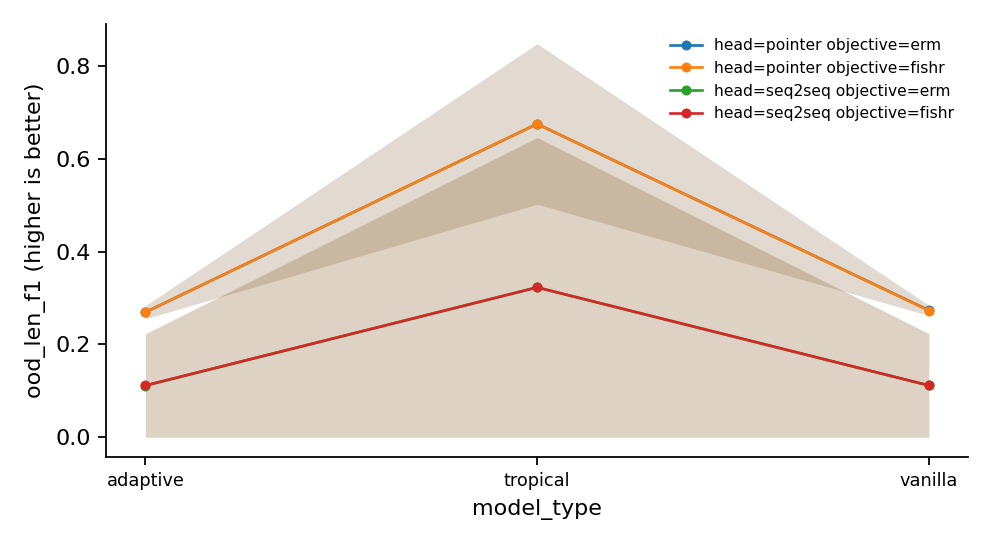
\includegraphics[width=\textwidth]{metric_ood_len_f1.png}
\caption{\texttt{ood\_len\_f1} against \texttt{model\_type}: the mean over seeds with a 95\% bootstrap CI, one line per combination of the other factors.}
\label{fig:ood_len_f1}
\end{figure}

{\small
\begin{longtable}{lllrlrrr}
\caption{\texttt{ood\_len\_f1} per cell: mean, 95\% bootstrap CI, SD, seeds, diverged runs.}\label{tab:summary-ood_len_f1}\\
\toprule
\texttt{model\_type} & \texttt{head} & \texttt{objective} & mean & 95\% CI & SD & $n$ & div.\\
\midrule
\endhead
adaptive & pointer & erm & 0.2693 & [0.255, 0.283] & 0.02 & 2 & 0\\
adaptive & pointer & fishr & 0.2693 & [0.255, 0.283] & 0.02 & 2 & 0\\
adaptive & seq2seq & erm & 0.1111 & [0, 0.222] & 0.157 & 2 & 0\\
adaptive & seq2seq & fishr & 0.1116 & [0, 0.223] & 0.158 & 2 & 0\\
tropical & pointer & erm & 0.6748 & [0.502, 0.848] & 0.244 & 2 & 0\\
tropical & pointer & fishr & 0.6748 & [0.502, 0.848] & 0.244 & 2 & 0\\
tropical & seq2seq & erm & 0.3228 & [0, 0.646] & 0.456 & 2 & 0\\
tropical & seq2seq & fishr & 0.3228 & [0, 0.646] & 0.456 & 2 & 0\\
vanilla & pointer & erm & 0.2734 & [0.262, 0.285] & 0.0157 & 2 & 0\\
vanilla & pointer & fishr & 0.2728 & [0.262, 0.283] & 0.0149 & 2 & 0\\
vanilla & seq2seq & erm & 0.1116 & [0, 0.223] & 0.158 & 2 & 0\\
vanilla & seq2seq & fishr & 0.1116 & [0, 0.223] & 0.158 & 2 & 0\\
\bottomrule
\end{longtable}
}

{\small
\begin{longtable}{lllrrrl}
\caption{\texttt{ood\_len\_f1}: each level of \texttt{model\_type} against its control (vanilla), within each combination of the other factors. rank: Wilcoxon signed-rank by seed, Holm.}\label{tab:control-ood_len_f1}\\
\toprule
\texttt{model\_type} & \texttt{head} & \texttt{objective} & difference & 95\% CI & $p$ & \\
\midrule
\endhead
adaptive & pointer & erm & -0.004152 & [-0.00715, -0.00115] & 1.0000 & \\
tropical & pointer & erm & 0.4013 & [0.24, 0.563] & 1.0000 & \\
adaptive & pointer & fishr & -0.003576 & [-0.00715, 0] & 1.0000 & \\
tropical & pointer & fishr & 0.4019 & [0.24, 0.564] & 1.0000 & \\
adaptive & seq2seq & erm & $-4.769\times10^{-4}$ & [$-9.54\times10^{-4}$, 0] & 1.0000 & \\
tropical & seq2seq & erm & 0.2112 & [0, 0.422] & 1.0000 & \\
adaptive & seq2seq & fishr & 0 & [0, 0] & -- & \\
tropical & seq2seq & fishr & 0.2112 & [0, 0.422] & 1.0000 & \\
\bottomrule
\end{longtable}
}


{\small
\begin{longtable}{lrrrl}
\caption{\texttt{ood\_len\_f1}: paired contrasts by seed, Holm-corrected across the cells. rank: Wilcoxon signed-rank by seed, Holm.}\label{tab:paired-ood_len_f1}\\
\toprule
contrast (within) & difference & 95\% CI & $p$ & \\
\midrule
\endhead
\makecell[l]{head: pointer - seq2seq\\\footnotesize model\_type=adaptive objective=erm } & 0.1582 & [-1.43, 1.75] & 1.0000 & \\
\makecell[l]{head: pointer - seq2seq\\\footnotesize model\_type=adaptive objective=fishr } & 0.1577 & [-1.44, 1.76] & 1.0000 & \\
\makecell[l]{head: pointer - seq2seq\\\footnotesize model\_type=tropical objective=erm } & 0.352 & [-5.94, 6.65] & 1.0000 & \\
\makecell[l]{head: pointer - seq2seq\\\footnotesize model\_type=tropical objective=fishr } & 0.352 & [-5.94, 6.65] & 1.0000 & \\
\makecell[l]{head: pointer - seq2seq\\\footnotesize model\_type=vanilla objective=erm } & 0.1618 & [-1.4, 1.72] & 1.0000 & \\
\makecell[l]{head: pointer - seq2seq\\\footnotesize model\_type=vanilla objective=fishr } & 0.1613 & [-1.39, 1.71] & 1.0000 & \\
\makecell[l]{objective: fishr - erm\\\footnotesize model\_type=adaptive head=pointer } & 0 & [--, --] & -- & \\
\makecell[l]{objective: fishr - erm\\\footnotesize model\_type=adaptive head=seq2seq } & $4.769\times10^{-4}$ & [-0.00558, 0.00654] & 1.0000 & \\
\makecell[l]{objective: fishr - erm\\\footnotesize model\_type=tropical head=pointer } & 0 & [--, --] & -- & \\
\makecell[l]{objective: fishr - erm\\\footnotesize model\_type=tropical head=seq2seq } & 0 & [--, --] & -- & \\
\makecell[l]{objective: fishr - erm\\\footnotesize model\_type=vanilla head=pointer } & $-5.760\times10^{-4}$ & [-0.0079, 0.00674] & 1.0000 & \\
\makecell[l]{objective: fishr - erm\\\footnotesize model\_type=vanilla head=seq2seq } & 0 & [--, --] & -- & \\
\bottomrule
\end{longtable}
}

\clearpage
\appendix
\section{Other metrics}
\subsection{\texttt{ood\_len\_exact}}
\begin{figure}[tbp]
\centering
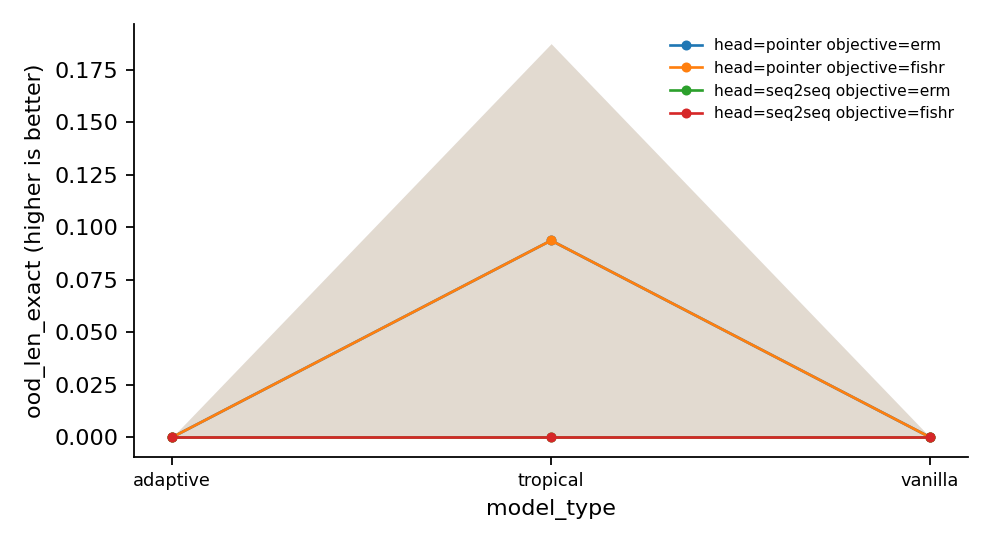
\includegraphics[width=\textwidth]{metric_ood_len_exact.png}
\caption{\texttt{ood\_len\_exact} against \texttt{model\_type}: the mean over seeds with a 95\% bootstrap CI, one line per combination of the other factors.}
\label{fig:ood_len_exact}
\end{figure}

{\small
\begin{longtable}{lllrlrrr}
\caption{\texttt{ood\_len\_exact} per cell: mean, 95\% bootstrap CI, SD, seeds, diverged runs.}\label{tab:summary-ood_len_exact}\\
\toprule
\texttt{model\_type} & \texttt{head} & \texttt{objective} & mean & 95\% CI & SD & $n$ & div.\\
\midrule
\endhead
adaptive & pointer & erm & 0 & [0, 0] & 0 & 2 & 0\\
adaptive & pointer & fishr & 0 & [0, 0] & 0 & 2 & 0\\
adaptive & seq2seq & erm & 0 & [0, 0] & 0 & 2 & 0\\
adaptive & seq2seq & fishr & 0 & [0, 0] & 0 & 2 & 0\\
tropical & pointer & erm & 0.09375 & [0, 0.188] & 0.133 & 2 & 0\\
tropical & pointer & fishr & 0.09375 & [0, 0.188] & 0.133 & 2 & 0\\
tropical & seq2seq & erm & 0 & [0, 0] & 0 & 2 & 0\\
tropical & seq2seq & fishr & 0 & [0, 0] & 0 & 2 & 0\\
vanilla & pointer & erm & 0 & [0, 0] & 0 & 2 & 0\\
vanilla & pointer & fishr & 0 & [0, 0] & 0 & 2 & 0\\
vanilla & seq2seq & erm & 0 & [0, 0] & 0 & 2 & 0\\
vanilla & seq2seq & fishr & 0 & [0, 0] & 0 & 2 & 0\\
\bottomrule
\end{longtable}
}

{\small
\begin{longtable}{lllrrrl}
\caption{\texttt{ood\_len\_exact}: each level of \texttt{model\_type} against its control (vanilla), within each combination of the other factors. rank: Wilcoxon signed-rank by seed, Holm.}\label{tab:control-ood_len_exact}\\
\toprule
\texttt{model\_type} & \texttt{head} & \texttt{objective} & difference & 95\% CI & $p$ & \\
\midrule
\endhead
adaptive & pointer & erm & 0 & [0, 0] & -- & \\
tropical & pointer & erm & 0.09375 & [0, 0.188] & 1.0000 & \\
adaptive & pointer & fishr & 0 & [0, 0] & -- & \\
tropical & pointer & fishr & 0.09375 & [0, 0.188] & 1.0000 & \\
adaptive & seq2seq & erm & 0 & [0, 0] & -- & \\
tropical & seq2seq & erm & 0 & [0, 0] & -- & \\
adaptive & seq2seq & fishr & 0 & [0, 0] & -- & \\
tropical & seq2seq & fishr & 0 & [0, 0] & -- & \\
\bottomrule
\end{longtable}
}


{\small
\begin{longtable}{lrrrl}
\caption{\texttt{ood\_len\_exact}: paired contrasts by seed, Holm-corrected across the cells. rank: Wilcoxon signed-rank by seed, Holm.}\label{tab:paired-ood_len_exact}\\
\toprule
contrast (within) & difference & 95\% CI & $p$ & \\
\midrule
\endhead
\makecell[l]{head: pointer - seq2seq\\\footnotesize model\_type=adaptive objective=erm } & 0 & [--, --] & -- & \\
\makecell[l]{head: pointer - seq2seq\\\footnotesize model\_type=adaptive objective=fishr } & 0 & [--, --] & -- & \\
\makecell[l]{head: pointer - seq2seq\\\footnotesize model\_type=tropical objective=erm } & 0.09375 & [-1.1, 1.28] & 1.0000 & \\
\makecell[l]{head: pointer - seq2seq\\\footnotesize model\_type=tropical objective=fishr } & 0.09375 & [-1.1, 1.28] & 1.0000 & \\
\makecell[l]{head: pointer - seq2seq\\\footnotesize model\_type=vanilla objective=erm } & 0 & [--, --] & -- & \\
\makecell[l]{head: pointer - seq2seq\\\footnotesize model\_type=vanilla objective=fishr } & 0 & [--, --] & -- & \\
\makecell[l]{objective: fishr - erm\\\footnotesize model\_type=adaptive head=pointer } & 0 & [--, --] & -- & \\
\makecell[l]{objective: fishr - erm\\\footnotesize model\_type=adaptive head=seq2seq } & 0 & [--, --] & -- & \\
\makecell[l]{objective: fishr - erm\\\footnotesize model\_type=tropical head=pointer } & 0 & [--, --] & -- & \\
\makecell[l]{objective: fishr - erm\\\footnotesize model\_type=tropical head=seq2seq } & 0 & [--, --] & -- & \\
\makecell[l]{objective: fishr - erm\\\footnotesize model\_type=vanilla head=pointer } & 0 & [--, --] & -- & \\
\makecell[l]{objective: fishr - erm\\\footnotesize model\_type=vanilla head=seq2seq } & 0 & [--, --] & -- & \\
\bottomrule
\end{longtable}
}

\subsection{\texttt{ood\_val\_f1}}
\begin{figure}[tbp]
\centering
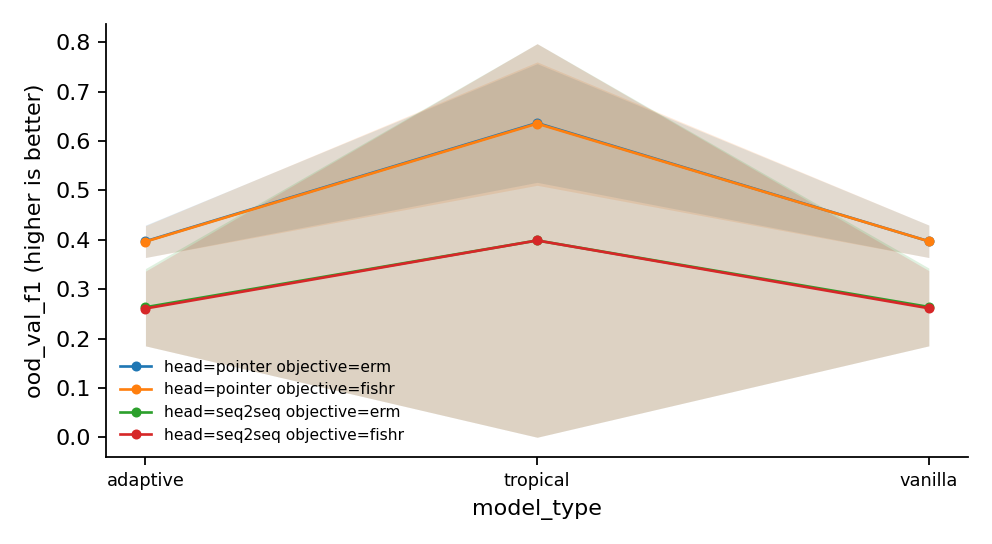
\includegraphics[width=\textwidth]{metric_ood_val_f1.png}
\caption{\texttt{ood\_val\_f1} against \texttt{model\_type}: the mean over seeds with a 95\% bootstrap CI, one line per combination of the other factors.}
\label{fig:ood_val_f1}
\end{figure}

{\small
\begin{longtable}{lllrlrrr}
\caption{\texttt{ood\_val\_f1} per cell: mean, 95\% bootstrap CI, SD, seeds, diverged runs.}\label{tab:summary-ood_val_f1}\\
\toprule
\texttt{model\_type} & \texttt{head} & \texttt{objective} & mean & 95\% CI & SD & $n$ & div.\\
\midrule
\endhead
adaptive & pointer & erm & 0.3971 & [0.364, 0.43] & 0.0465 & 2 & 0\\
adaptive & pointer & fishr & 0.3964 & [0.364, 0.429] & 0.0455 & 2 & 0\\
adaptive & seq2seq & erm & 0.2635 & [0.185, 0.342] & 0.111 & 2 & 0\\
adaptive & seq2seq & fishr & 0.2608 & [0.185, 0.337] & 0.107 & 2 & 0\\
tropical & pointer & erm & 0.6368 & [0.517, 0.757] & 0.17 & 2 & 0\\
tropical & pointer & fishr & 0.6355 & [0.511, 0.761] & 0.177 & 2 & 0\\
tropical & seq2seq & erm & 0.3987 & [0, 0.797] & 0.564 & 2 & 0\\
tropical & seq2seq & fishr & 0.3987 & [0, 0.797] & 0.564 & 2 & 0\\
vanilla & pointer & erm & 0.3971 & [0.364, 0.43] & 0.0465 & 2 & 0\\
vanilla & pointer & fishr & 0.3971 & [0.364, 0.43] & 0.0465 & 2 & 0\\
vanilla & seq2seq & erm & 0.264 & [0.185, 0.343] & 0.111 & 2 & 0\\
vanilla & seq2seq & fishr & 0.2614 & [0.185, 0.338] & 0.108 & 2 & 0\\
\bottomrule
\end{longtable}
}

{\small
\begin{longtable}{lllrrrl}
\caption{\texttt{ood\_val\_f1}: each level of \texttt{model\_type} against its control (vanilla), within each combination of the other factors. parametric: Dunnett vs control.}\label{tab:control-ood_val_f1}\\
\toprule
\texttt{model\_type} & \texttt{head} & \texttt{objective} & difference & 95\% CI & $p$ & \\
\midrule
\endhead
adaptive & pointer & erm & 0 & [-0.409, 0.409] & 1.0000 & \\
tropical & pointer & erm & 0.2397 & [-0.169, 0.649] & 0.1707 & \\
adaptive & pointer & fishr & $-6.676\times10^{-4}$ & [-0.423, 0.422] & 1.0000 & \\
tropical & pointer & fishr & 0.2385 & [-0.184, 0.661] & 0.1842 & \\
adaptive & seq2seq & erm & $-5.425\times10^{-4}$ & [-1.31, 1.31] & 1.0000 & \\
tropical & seq2seq & erm & 0.1347 & [-1.18, 1.45] & 0.8953 & \\
adaptive & seq2seq & fishr & $-5.358\times10^{-4}$ & [-1.31, 1.31] & 1.0000 & \\
tropical & seq2seq & fishr & 0.1374 & [-1.17, 1.45] & 0.8911 & \\
\bottomrule
\end{longtable}
}


{\small
\begin{longtable}{lrrrl}
\caption{\texttt{ood\_val\_f1}: paired contrasts by seed, Holm-corrected across the cells. parametric: paired t-test by seed, Holm.}\label{tab:paired-ood_val_f1}\\
\toprule
contrast (within) & difference & 95\% CI & $p$ & \\
\midrule
\endhead
\makecell[l]{head: pointer - seq2seq\\\footnotesize model\_type=adaptive objective=erm } & 0.1336 & [-0.444, 0.711] & 1.0000 & \\
\makecell[l]{head: pointer - seq2seq\\\footnotesize model\_type=adaptive objective=fishr } & 0.1355 & [-0.417, 0.688] & 1.0000 & \\
\makecell[l]{head: pointer - seq2seq\\\footnotesize model\_type=tropical objective=erm } & 0.238 & [-6.36, 6.83] & 1.0000 & \\
\makecell[l]{head: pointer - seq2seq\\\footnotesize model\_type=tropical objective=fishr } & 0.2368 & [-6.42, 6.89] & 1.0000 & \\
\makecell[l]{head: pointer - seq2seq\\\footnotesize model\_type=vanilla objective=erm } & 0.133 & [-0.451, 0.717] & 1.0000 & \\
\makecell[l]{head: pointer - seq2seq\\\footnotesize model\_type=vanilla objective=fishr } & 0.1357 & [-0.415, 0.686] & 1.0000 & \\
\makecell[l]{objective: fishr - erm\\\footnotesize model\_type=adaptive head=pointer } & $-6.676\times10^{-4}$ & [-0.00915, 0.00781] & 1.0000 & \\
\makecell[l]{objective: fishr - erm\\\footnotesize model\_type=adaptive head=seq2seq } & -0.002632 & [-0.0361, 0.0308] & 1.0000 & \\
\makecell[l]{objective: fishr - erm\\\footnotesize model\_type=tropical head=pointer } & -0.001252 & [-0.0617, 0.0591] & 1.0000 & \\
\makecell[l]{objective: fishr - erm\\\footnotesize model\_type=tropical head=seq2seq } & 0 & [--, --] & -- & \\
\makecell[l]{objective: fishr - erm\\\footnotesize model\_type=vanilla head=pointer } & 0 & [--, --] & -- & \\
\makecell[l]{objective: fishr - erm\\\footnotesize model\_type=vanilla head=seq2seq } & -0.002639 & [-0.0362, 0.0309] & 1.0000 & \\
\bottomrule
\end{longtable}
}

\subsection{\texttt{id\_f1}}
\begin{figure}[tbp]
\centering
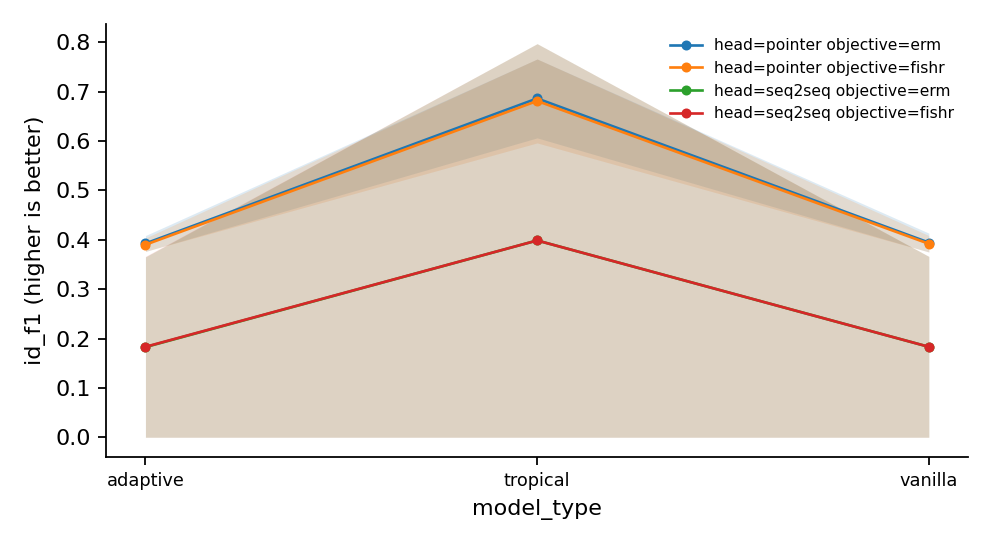
\includegraphics[width=\textwidth]{metric_id_f1.png}
\caption{\texttt{id\_f1} against \texttt{model\_type}: the mean over seeds with a 95\% bootstrap CI, one line per combination of the other factors.}
\label{fig:id_f1}
\end{figure}

{\small
\begin{longtable}{lllrlrrr}
\caption{\texttt{id\_f1} per cell: mean, 95\% bootstrap CI, SD, seeds, diverged runs.}\label{tab:summary-id_f1}\\
\toprule
\texttt{model\_type} & \texttt{head} & \texttt{objective} & mean & 95\% CI & SD & $n$ & div.\\
\midrule
\endhead
adaptive & pointer & erm & 0.3926 & [0.377, 0.409] & 0.0227 & 2 & 0\\
adaptive & pointer & fishr & 0.3901 & [0.377, 0.404] & 0.0192 & 2 & 0\\
adaptive & seq2seq & erm & 0.1827 & [0, 0.365] & 0.258 & 2 & 0\\
adaptive & seq2seq & fishr & 0.1832 & [0, 0.366] & 0.259 & 2 & 0\\
tropical & pointer & erm & 0.6865 & [0.607, 0.766] & 0.113 & 2 & 0\\
tropical & pointer & fishr & 0.6814 & [0.596, 0.766] & 0.12 & 2 & 0\\
tropical & seq2seq & erm & 0.3987 & [0, 0.797] & 0.564 & 2 & 0\\
tropical & seq2seq & fishr & 0.3987 & [0, 0.797] & 0.564 & 2 & 0\\
vanilla & pointer & erm & 0.3945 & [0.375, 0.414] & 0.027 & 2 & 0\\
vanilla & pointer & fishr & 0.392 & [0.375, 0.409] & 0.0235 & 2 & 0\\
vanilla & seq2seq & erm & 0.1832 & [0, 0.366] & 0.259 & 2 & 0\\
vanilla & seq2seq & fishr & 0.1832 & [0, 0.366] & 0.259 & 2 & 0\\
\bottomrule
\end{longtable}
}

{\small
\begin{longtable}{lllrrrl}
\caption{\texttt{id\_f1}: each level of \texttt{model\_type} against its control (vanilla), within each combination of the other factors. rank: Wilcoxon signed-rank by seed, Holm.}\label{tab:control-id_f1}\\
\toprule
\texttt{model\_type} & \texttt{head} & \texttt{objective} & difference & 95\% CI & $p$ & \\
\midrule
\endhead
adaptive & pointer & erm & -0.001876 & [-0.00491, 0.00116] & 1.0000 & \\
tropical & pointer & erm & 0.2921 & [0.193, 0.391] & 1.0000 & \\
adaptive & pointer & fishr & -0.001892 & [-0.00494, 0.00116] & 1.0000 & \\
tropical & pointer & fishr & 0.2894 & [0.188, 0.391] & 1.0000 & \\
adaptive & seq2seq & erm & $-5.673\times10^{-4}$ & [-0.00113, 0] & 1.0000 & \\
tropical & seq2seq & erm & 0.2155 & [0, 0.431] & 1.0000 & \\
adaptive & seq2seq & fishr & 0 & [0, 0] & -- & \\
tropical & seq2seq & fishr & 0.2155 & [0, 0.431] & 1.0000 & \\
\bottomrule
\end{longtable}
}


{\small
\begin{longtable}{lrrrl}
\caption{\texttt{id\_f1}: paired contrasts by seed, Holm-corrected across the cells. rank: Wilcoxon signed-rank by seed, Holm.}\label{tab:paired-id_f1}\\
\toprule
contrast (within) & difference & 95\% CI & $p$ & \\
\midrule
\endhead
\makecell[l]{head: pointer - seq2seq\\\footnotesize model\_type=adaptive objective=erm } & 0.2099 & [-1.91, 2.33] & 1.0000 & \\
\makecell[l]{head: pointer - seq2seq\\\footnotesize model\_type=adaptive objective=fishr } & 0.2069 & [-1.95, 2.36] & 1.0000 & \\
\makecell[l]{head: pointer - seq2seq\\\footnotesize model\_type=tropical objective=erm } & 0.2878 & [-5.79, 6.37] & 1.0000 & \\
\makecell[l]{head: pointer - seq2seq\\\footnotesize model\_type=tropical objective=fishr } & 0.2827 & [-5.86, 6.43] & 1.0000 & \\
\makecell[l]{head: pointer - seq2seq\\\footnotesize model\_type=vanilla objective=erm } & 0.2113 & [-1.87, 2.3] & 1.0000 & \\
\makecell[l]{head: pointer - seq2seq\\\footnotesize model\_type=vanilla objective=fishr } & 0.2088 & [-1.91, 2.33] & 1.0000 & \\
\makecell[l]{objective: fishr - erm\\\footnotesize model\_type=adaptive head=pointer } & -0.002471 & [-0.0339, 0.0289] & 1.0000 & \\
\makecell[l]{objective: fishr - erm\\\footnotesize model\_type=adaptive head=seq2seq } & $5.673\times10^{-4}$ & [-0.00664, 0.00778] & 1.0000 & \\
\makecell[l]{objective: fishr - erm\\\footnotesize model\_type=tropical head=pointer } & -0.005111 & [-0.07, 0.0598] & 1.0000 & \\
\makecell[l]{objective: fishr - erm\\\footnotesize model\_type=tropical head=seq2seq } & 0 & [--, --] & -- & \\
\makecell[l]{objective: fishr - erm\\\footnotesize model\_type=vanilla head=pointer } & -0.002456 & [-0.0337, 0.0287] & 1.0000 & \\
\makecell[l]{objective: fishr - erm\\\footnotesize model\_type=vanilla head=seq2seq } & 0 & [--, --] & -- & \\
\bottomrule
\end{longtable}
}

\subsection{\texttt{id\_exact}}
\begin{figure}[tbp]
\centering
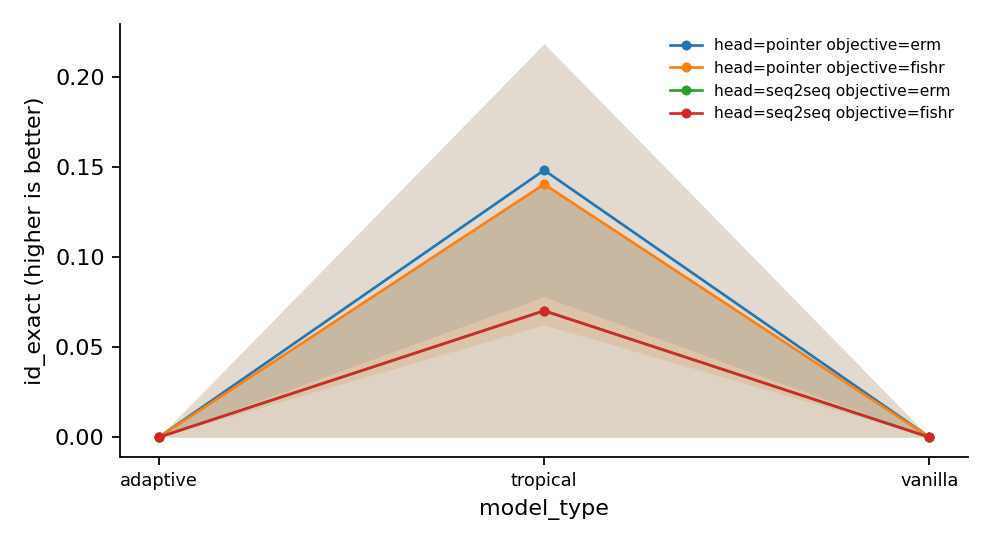
\includegraphics[width=\textwidth]{metric_id_exact.png}
\caption{\texttt{id\_exact} against \texttt{model\_type}: the mean over seeds with a 95\% bootstrap CI, one line per combination of the other factors.}
\label{fig:id_exact}
\end{figure}

{\small
\begin{longtable}{lllrlrrr}
\caption{\texttt{id\_exact} per cell: mean, 95\% bootstrap CI, SD, seeds, diverged runs.}\label{tab:summary-id_exact}\\
\toprule
\texttt{model\_type} & \texttt{head} & \texttt{objective} & mean & 95\% CI & SD & $n$ & div.\\
\midrule
\endhead
adaptive & pointer & erm & 0 & [0, 0] & 0 & 2 & 0\\
adaptive & pointer & fishr & 0 & [0, 0] & 0 & 2 & 0\\
adaptive & seq2seq & erm & 0 & [0, 0] & 0 & 2 & 0\\
adaptive & seq2seq & fishr & 0 & [0, 0] & 0 & 2 & 0\\
tropical & pointer & erm & 0.1484 & [0.0781, 0.219] & 0.0994 & 2 & 0\\
tropical & pointer & fishr & 0.1406 & [0.0625, 0.219] & 0.11 & 2 & 0\\
tropical & seq2seq & erm & 0.07031 & [0, 0.141] & 0.0994 & 2 & 0\\
tropical & seq2seq & fishr & 0.07031 & [0, 0.141] & 0.0994 & 2 & 0\\
vanilla & pointer & erm & 0 & [0, 0] & 0 & 2 & 0\\
vanilla & pointer & fishr & 0 & [0, 0] & 0 & 2 & 0\\
vanilla & seq2seq & erm & 0 & [0, 0] & 0 & 2 & 0\\
vanilla & seq2seq & fishr & 0 & [0, 0] & 0 & 2 & 0\\
\bottomrule
\end{longtable}
}

{\small
\begin{longtable}{lllrrrl}
\caption{\texttt{id\_exact}: each level of \texttt{model\_type} against its control (vanilla), within each combination of the other factors. rank: Wilcoxon signed-rank by seed, Holm.}\label{tab:control-id_exact}\\
\toprule
\texttt{model\_type} & \texttt{head} & \texttt{objective} & difference & 95\% CI & $p$ & \\
\midrule
\endhead
adaptive & pointer & erm & 0 & [0, 0] & -- & \\
tropical & pointer & erm & 0.1484 & [0.0781, 0.219] & 0.5000 & \\
adaptive & pointer & fishr & 0 & [0, 0] & -- & \\
tropical & pointer & fishr & 0.1406 & [0.0625, 0.219] & 0.5000 & \\
adaptive & seq2seq & erm & 0 & [0, 0] & -- & \\
tropical & seq2seq & erm & 0.07031 & [0, 0.141] & 1.0000 & \\
adaptive & seq2seq & fishr & 0 & [0, 0] & -- & \\
tropical & seq2seq & fishr & 0.07031 & [0, 0.141] & 1.0000 & \\
\bottomrule
\end{longtable}
}


{\small
\begin{longtable}{lrrrl}
\caption{\texttt{id\_exact}: paired contrasts by seed, Holm-corrected across the cells. rank: Wilcoxon signed-rank by seed, Holm.}\label{tab:paired-id_exact}\\
\toprule
contrast (within) & difference & 95\% CI & $p$ & \\
\midrule
\endhead
\makecell[l]{head: pointer - seq2seq\\\footnotesize model\_type=adaptive objective=erm } & 0 & [--, --] & -- & \\
\makecell[l]{head: pointer - seq2seq\\\footnotesize model\_type=adaptive objective=fishr } & 0 & [--, --] & -- & \\
\makecell[l]{head: pointer - seq2seq\\\footnotesize model\_type=tropical objective=erm } & 0.07812 & [-1.71, 1.86] & 1.0000 & \\
\makecell[l]{head: pointer - seq2seq\\\footnotesize model\_type=tropical objective=fishr } & 0.07031 & [-1.82, 1.96] & 1.0000 & \\
\makecell[l]{head: pointer - seq2seq\\\footnotesize model\_type=vanilla objective=erm } & 0 & [--, --] & -- & \\
\makecell[l]{head: pointer - seq2seq\\\footnotesize model\_type=vanilla objective=fishr } & 0 & [--, --] & -- & \\
\makecell[l]{objective: fishr - erm\\\footnotesize model\_type=adaptive head=pointer } & 0 & [--, --] & -- & \\
\makecell[l]{objective: fishr - erm\\\footnotesize model\_type=adaptive head=seq2seq } & 0 & [--, --] & -- & \\
\makecell[l]{objective: fishr - erm\\\footnotesize model\_type=tropical head=pointer } & -0.007812 & [-0.107, 0.0915] & 1.0000 & \\
\makecell[l]{objective: fishr - erm\\\footnotesize model\_type=tropical head=seq2seq } & 0 & [--, --] & -- & \\
\makecell[l]{objective: fishr - erm\\\footnotesize model\_type=vanilla head=pointer } & 0 & [--, --] & -- & \\
\makecell[l]{objective: fishr - erm\\\footnotesize model\_type=vanilla head=seq2seq } & 0 & [--, --] & -- & \\
\bottomrule
\end{longtable}
}


\section{Curves}
\begin{figure}[tbp]
\centering
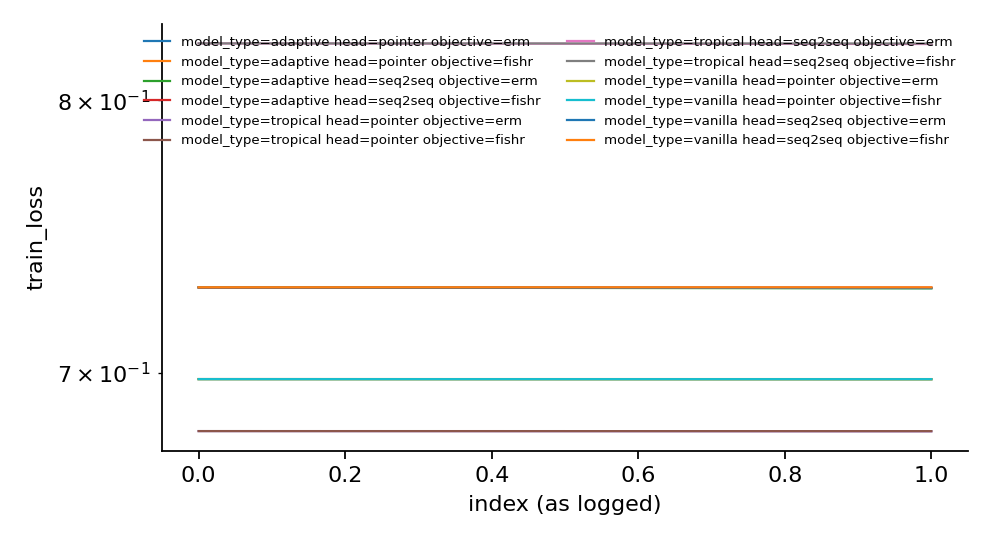
\includegraphics[width=\textwidth]{curve_train_loss.png}
\caption{\texttt{train\_loss}, the mean over seeds per cell.}
\label{fig:curve-1}
\end{figure}
\begin{figure}[tbp]
\centering
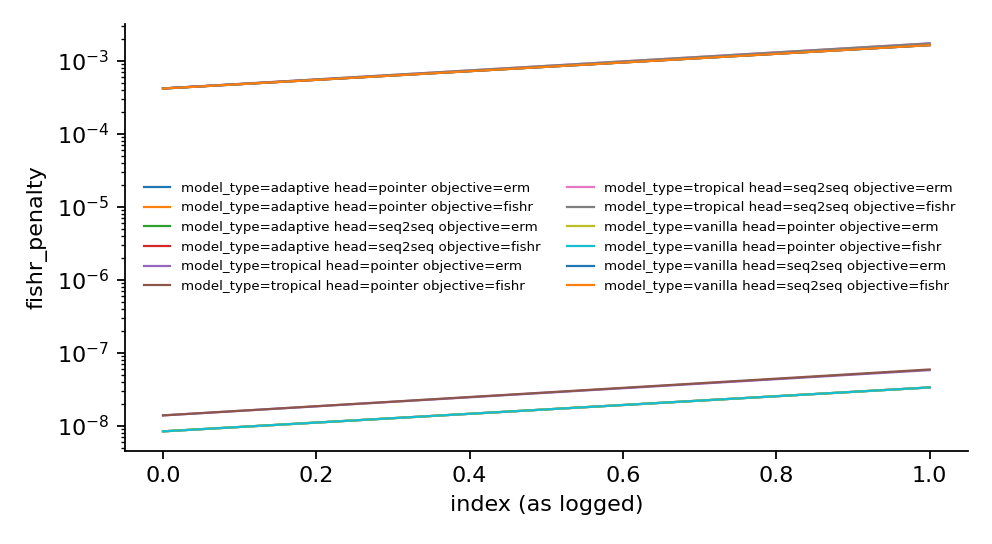
\includegraphics[width=\textwidth]{curve_fishr_penalty.png}
\caption{\texttt{fishr\_penalty}, the mean over seeds per cell.}
\label{fig:curve-2}
\end{figure}
\begin{figure}[tbp]
\centering
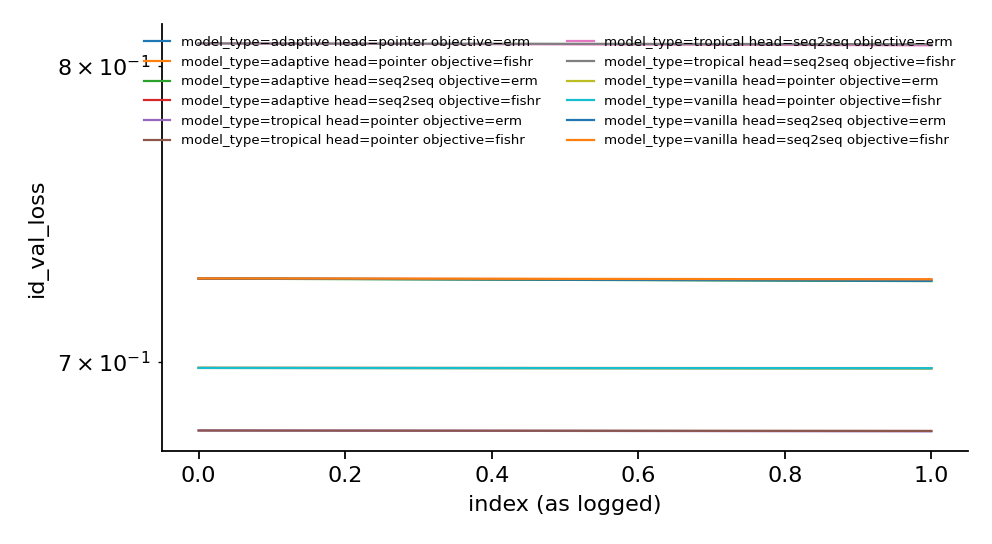
\includegraphics[width=\textwidth]{curve_id_val_loss.png}
\caption{\texttt{id\_val\_loss}, the mean over seeds per cell.}
\label{fig:curve-3}
\end{figure}

\section{Configuration}
The base configuration every run shares (frozen hash \texttt{1a157652ea23}); factor levels are in \autoref{tab:summary-ood_len_f1}.
{\footnotesize
\begin{verbatim}
task:
  name: KnapsackDataset
  value_range:
  - 1
  - 10
  target_range:
  - 10
  - 20
  weight_range:
  - 1
  - 10
  adversarial_range:
  - 10
  - 30
  noise_prob: 0.0
data:
  train_lengths:
  - 4
  - 5
  ood_lengths:
  - 8
  n_per_length: 64
  n_eval_per_length: 32
  curve_eval_limit: 16
model:
  d_model: 64
  n_heads: 2
  num_layers: 1
  dropout: 0.0
  tropical_impl: legacy
optim:
  lr: 0.0001
  epochs: 2
  batch_size: 16
  eval_batch_size: 256
fishr:
  lambda: 10.0
  ema: 0.95
  anneal_iters: 2
  reset_optimizer: true
\end{verbatim}
}
Store: \texttt{campaigns/tropical/dry\_run/results}.
\end{document}